
%%
\documentclass[sigconf]{acmart}
\usepackage{algorithm}
\usepackage{algpseudocode}
\usepackage{siunitx}
\usepackage{microtype}
\usepackage[inline]{enumitem}
%%
\AtBeginDocument{%
  \providecommand\BibTeX{{%
    Bib\TeX}}}

\begin{document}

\title{TSS: Temporal Significance Scheduling for MX-Quantized LLM FFN Inference on CIM}


\begin{abstract}
    Compute-reduction methods for quantized Large Language Model (LLM) inference on Compute-in-Memory (CIM) architectures typically rely on fixed local masks, which preserve hardware regularity but yield a coarse quality-compute tradeoff. Conversely, attempts to improve model quality via flexible sparsity introduce spatial irregularity that severely conflicts with CIM's rigid execution constraints. To overcome this limitation, we propose \textbf{Temporal Significance Scheduling (TSS)}, a novel approach that utilizes an alternative significance signal to natively support regular hardware mapping. Rather than masking raw inputs spatially, we reinterpret the block-scale and element-level exponent metadata of the Microscaling (MX) representation as arrival-time signals within a Most Significant Digit (MSD)-first online-arithmetic stream. By temporally bounding operation horizons based on data significance, our method dynamically suppresses ineffectual computations without disrupting spatial regularity. We implement this scheduling via a two-plane Feed-Forward Network (FFN) micro-tile, mapping operations onto channel-parallel, block-serial online-arithmetic engines managed by a lightweight, narrow-integer control plane. Evaluations on Qwen3-0.6B with MXFP8 quantization demonstrate that TSS achieves a superior quality-compute tradeoff, maintaining near-dense baseline perplexity while executing only 50\% of the workload. Because block-serial latency is dictated by live-interval contraction rather than raw operation count, this compute reduction translates to a 22--25\% layer-wise FFN latency improvement, incurring minimal hardware overheads of only 0.3\% in area and ${\sim}$2.5\% in power. To ensure reproducibility, our transaction-level simulator and hardware evaluation framework are open-sourced anonymously.
\end{abstract}

\keywords{LLM Inference, Compute-in-Memory, MX Quantization, Temporal Scheduling}


\maketitle

% ===========================================================================
\section{Introduction}
\label{sec:intro}
% ===========================================================================

Inference in large language models (LLMs) is computationally dominated by feed-forward network (FFN) blocks~\cite{samsi2023words,lo2015roofline}. Compute-in-memory (CIM)~\cite{fujiwara20225,yu2021compute} architectures offer a natural execution substrate for accelerating quantized FFN projections by co-locating logic and storage. However, they impose a strict regularity constraint: execution schedules must map to fixed array structures with minimal runtime control divergence~\cite{jeong2023vegeta,mishra2021accelerating,ramachandran2025accelerating}.

Existing CIM-friendly compute-reduction methods typically enforce rigid local masks---such as structured $2{:}4$ sparsity patterns or static block pruning~\cite{10904702,9768124}---to preserve this regularity. While the resulting hardware is straightforward, the tradeoff between model quality and computational reduction is inherently coarse; at moderate sparsity ratios, perplexity degrades disproportionately relative to computational savings~\cite{harma2024effective,frantar2023sparsegpt}. The conventional remedy is to employ more flexible or data-dependent sparsity~\cite{jeong2023vegeta,mishra2021accelerating}. However, such approaches introduce additional metadata overhead, runtime irregularity, or require model retraining, thereby eroding the fundamental efficiency advantages of CIM~\cite{ramachandran2025accelerating}.

To overcome these limitations, this paper introduces \textbf{Temporal Significance Scheduling (TSS)}. Rather than increasing the complexity of spatial sparsity masks, we reframe the execution problem around \emph{significance-driven temporal truncation}. By refining the significance signal used to determine workload execution, our approach preserves a regular execution substrate while enabling the early termination of less critical operations. 

\textbf{Key observation.} Microscaling (MX) quantization~\cite{rouhani2023ocp}, increasingly adopted for low-precision LLM deployment~\cite{wang2025infir2,mishra2025recipes}, stores per-block scale exponents alongside quantized operands. These exponent fields natively encode the relative numerical significance of each block and, at a finer granularity, each element. When computation is structured as most-significant-digit (MSD)-first online arithmetic~\cite{villalba2011radix,huang2001fpga,zhao2016efficient}---where the most-significant digit of each partial product is emitted first---this metadata dictates \emph{when} each contribution accumulates in the output stream. Contributions with large combined exponents arrive early, whereas those with small exponents arrive late, contributing proportionally less to the final result under a fixed execution budget.

Numerically, this behavior aligns directly with significance aware computation and early termination~\cite{10454447,7783722}. Ordinarily, temporal truncation targets raw input operands~\cite{7783722} or generic variable precision datapaths~\cite{10454447}, which are often hostile to CIM regularity. In our setting, however, MX block- and element-level exponents first induce a temporal alignment across contributions. The hardware scheduler then retains only the most significant prefix of this aligned contribution stream. Consequently, our method acts as a hardware-friendly scheduling policy rather than a standalone truncation heuristic, enabling significance-ordered early termination on regular CIM arrays.

\begin{figure*}[htbp]
  \centering
  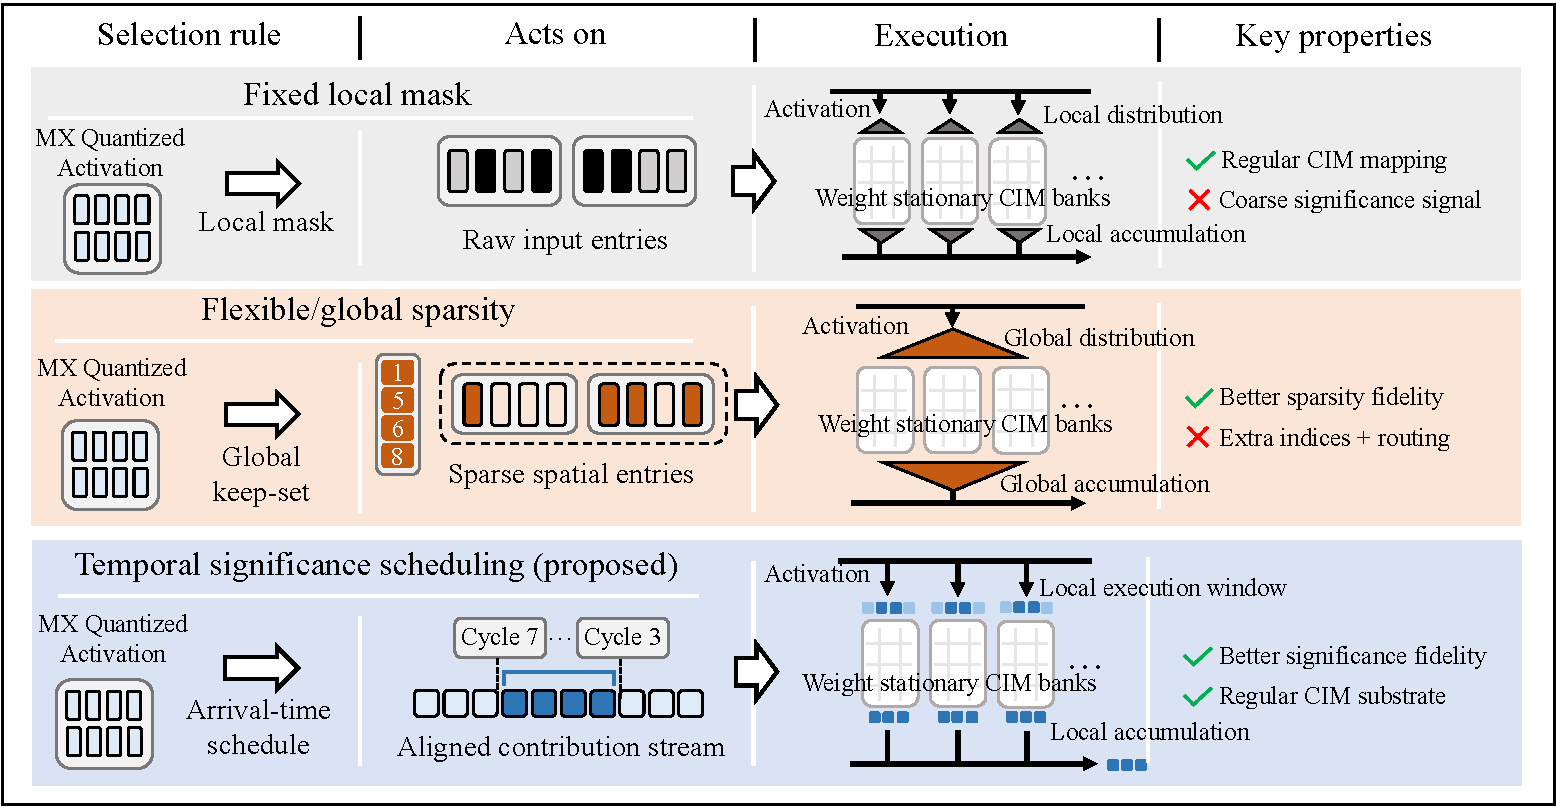
\includegraphics[width=0.9\textwidth]{figures/figure1.pdf}
  \vspace{-1mm}
  \caption{%
    Temporal significance scheduling: an improved significance signal for MX-quantized
    CIM FFN execution.}
  \label{fig:motivation}
  \vspace{-3mm}
\end{figure*}

As illustrated in Figure~\ref{fig:motivation}, our approach contrasts sharply with spatial sparsity techniques; rather than applying repeated local masks to raw inputs or global keep-sets to spatial entries, it operates by dynamically scheduling arrival times on aligned contribution streams.

\textbf{Temporal Significance Scheduling (TSS).}
Operationally, we formulate this abstraction to act directly on an aligned contribution stream. For every block--element pair, the hardware synthesizes an arrival index from existing MX metadata: the activation block-scale exponent, the weight block-scale exponent, and a per-element activation fine-delay code. After temporally aligning the streams, the scheduler applies a calibrated per-channel execution \emph{horizon} to dictate the execution depth. By restricting the digits emitted during MSD-first online multiplication, this mechanism enforces significance-ordered early termination while strictly preserving the underlying regular datapath. This single windowed schedule natively subsumes whole-block skipping, element suppression, and shortened block service intervals under a unified formulation.

\textbf{Contributions.}
This paper makes the following contributions:
\begin{enumerate}[nosep,leftmargin=1.2em]
  \item \textbf{A novel execution abstraction.} We introduce TSS, maximizing efficiency by applying significance-aware temporal truncation to aligned contribution streams using existing MX quantization metadata.
  \item \textbf{A regular hardware realization.} We propose a metadata-first, two-plane FFN micro-tile tailored for channel-parallel, block-serial online arithmetic. The control plane relies on lightweight integer logic to process metadata, ensuring the data plane remains a highly regular serial--parallel array.
  \item \textbf{An improved quality-efficiency tradeoff.} We demonstrate that TSS systematically outperforms activation-gated CIM baselines. Through layer-wise budget redistribution, our approach yields substantial reductions in FFN layer latency and executed operations while preserving baseline model perplexity.
  \item \textbf{Open-source simulation framework.} To facilitate future research, we open-source our bit-exact transaction-level model (TLM) and evaluation scripts.
\end{enumerate}

%In tended to adjust section seperation
%\raggedbottom


% ===========================================================================
\section{Background}
\label{sec:background}
% ===========================================================================

This section introduces the inference target, quantization context, and hardware-visible metadata leveraged by temporal significance scheduling.

% ---------------------------------------------------------------------------
\subsection{GLU-FFN Target}
\label{sec:bg:ffn}
% ---------------------------------------------------------------------------

Modern large language models typically employ gated linear unit (GLU) feed-forward networks (FFNs)~\cite{shazeer2020glu}:
\begin{equation}
  \mathbf{y}
  = W_{\mathrm{down}}\!\Bigl(
      \phi\!\bigl(W_{\mathrm{gate}}\,\mathbf{x}\bigr)
      \odot
      W_{\mathrm{up}}\,\mathbf{x}
    \Bigr),
  \label{eq:glu-ffn}
\end{equation}
where $\phi$ is the gating nonlinearity and $\odot$ denotes element-wise multiplication. The three dense projections ($W_{\mathrm{gate}}$, $W_{\mathrm{up}}$, $W_{\mathrm{down}}$) dominate inference costs, comprising roughly two-thirds of the model's parameters and total operations. 

This GLU structure is highly amenable to quantized compute-in-memory (CIM) execution. The large matrix--vector products exhibit regular, token-independent access patterns, while the point-wise gating operation can be evaluated locally between projection stages.

\begin{figure*}[htbp]
  \centering
  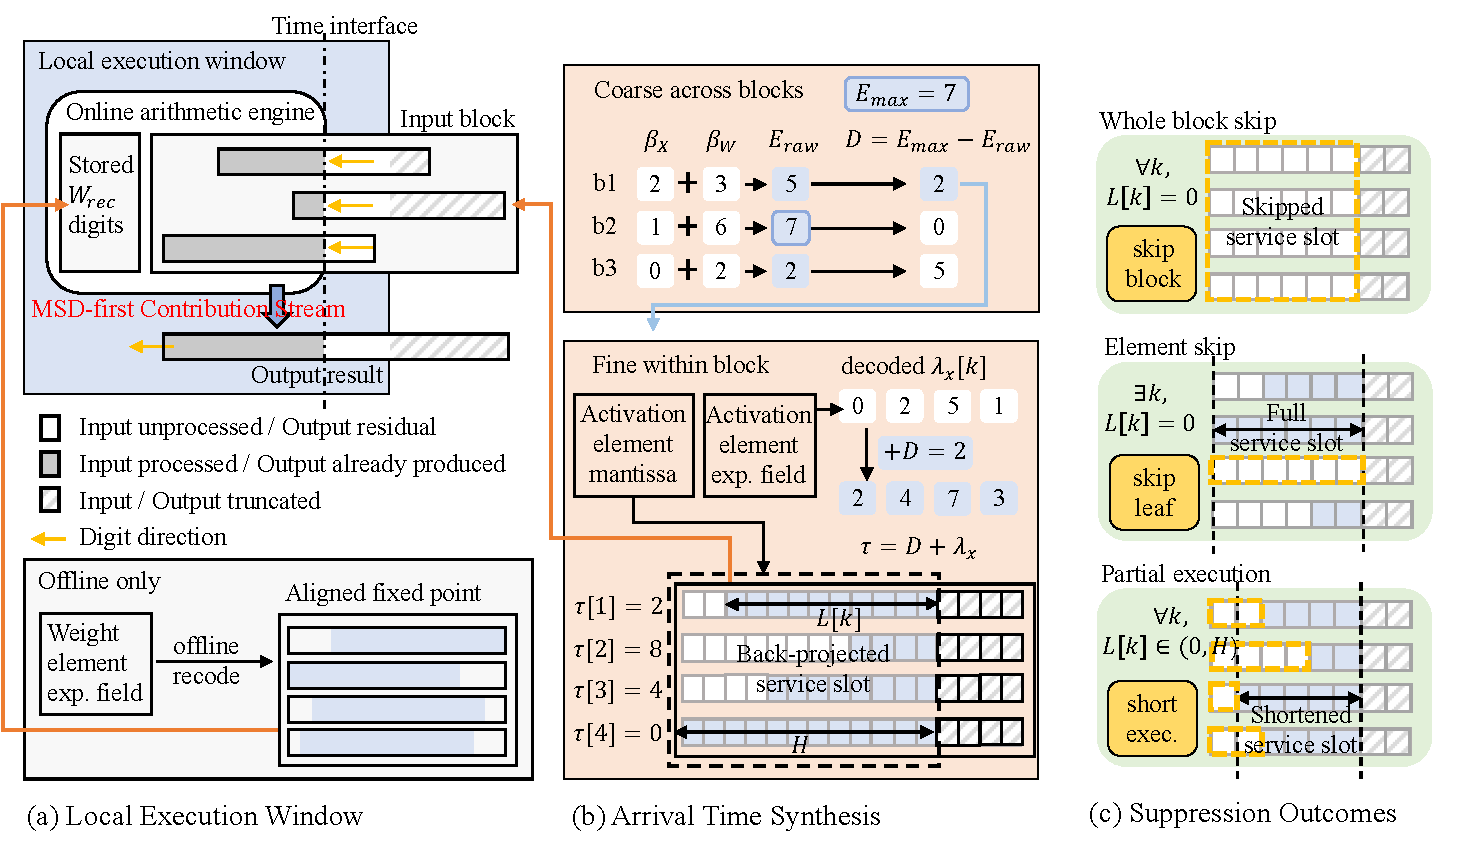
\includegraphics[width=0.8\textwidth]{figures/figure2.pdf}
  \caption{%
    \textbf{Local execution windows on aligned MSD-first contribution
    streams.}}
  \label{fig:concept}
\end{figure*}

% ---------------------------------------------------------------------------
\subsection{MX Quantization and Metadata}
\label{sec:bg:mx}
% ---------------------------------------------------------------------------

Microscaling (MX) quantization partitions tensors into fixed-size blocks (typically $K{=}32$)~\cite{rouhani2023ocp}, assigning a shared block-scale exponent to each. Within a block, individual elements are represented in low-precision floating-point formats. This two-level structure balances dynamic range and storage costs, aligning with emerging industry specifications~\cite{darvish2023shared,wang2025infir2,mishra2025recipes}.

TSS relies on four hardware-visible metadata quantities: (1) \textbf{Activation block-scale exponent} $\beta_x[n,b]$ (\emph{Native}): The standard, shared E8M0 exponent of activation block~$b$ for token~$n$.
(2) \textbf{Weight block-scale exponent} $\beta_w[p,c,b]$ (\emph{Native}): The shared E8M0 exponent of weight block~$b$ on path $p \in \{g, u\}$ for output channel~$c$.
(3) \textbf{Activation fine-delay code} $\lambda_x[n,b,k]$ (\emph{Derived}): A per-element modifier, extracted directly from the native MXFP element exponent to refine intra-block significance ordering. 
(4) \textbf{Calibrated horizon} $H[p,c]$ (\emph{Introduced}): An offline-calibrated per-path and per-channel scalar that explicitly bounds the execution budget.




% ---------------------------------------------------------------------------
\subsection{Online Arithmetic Context}
\label{sec:bg:online}
% ---------------------------------------------------------------------------

CIM arrays designed for low-precision quantized inference can be structured to emit partial products in a most-significant-digit-first (MSD-first) order using online arithmetic~\cite{villalba2011radix,huang2001fpga,zhao2016efficient}. Under this regime, each multiplier leaf generates output digits sequentially from the most significant position, while a reduction tree accumulates these streams across the block. 

TSS exploits a key property of this temporal data flow: the \emph{numerical significance of a digit is monotonically non-increasing} relative to its emission order. Consequently, earlier digits contribute exponentially more to the accumulated value than later ones.

When operand blocks possess different combined exponents, their contribution streams must be \emph{aligned} prior to accumulation---mirroring conventional floating-point addition, but distributed temporally. A block with a larger combined exponent begins contributing at an earlier time step, effectively delaying the processing of blocks with smaller exponents. Through this temporal alignment, standard exponent metadata fundamentally acts as an arrival-time signal for the hardware.


%========================================================
\section{Temporal Significance Scheduling}
\label{sec:method}
%========================================================

This section introduces the core abstractions of Temporal Significance Scheduling (TSS).
For notational clarity, the token, projection path (e.g., gate or up), and target channel indices are omitted throughout this discussion. 
The runtime control logic evaluates exactly four hardware-visible quantities across blocks~$b$ and intra-block elements~$k$:
\begin{itemize*}
  \item $\beta_x[b]$\,: activation block-scale exponent,
  \item $\beta_w[b]$\,: weight block-scale exponent,
  \item $\lambda_x[b,k]$\,: activation-side fine-delay code,
  \item $H$\,: calibrated per-channel horizon.
\end{itemize*}

These variables are narrow integer fields that are either natively present within or efficiently derivable from the MX representation.
Because the weight-element exponent is folded offline into the stored, recoded weights, it requires no runtime resolution.
Consequently, runtime scheduling relies \textbf{strictly on metadata}: it entails only field readouts, narrow integer addition and subtraction, maximum reductions, and comparisons, entirely eliminating the requirement for a floating-point datapath.

%% --------------------------------------------------
\subsection{Online Arrival-Time Synthesis}
\label{sec:arrival}

Block-scale metadata establish a coarse relative timing across blocks. As illustrated in Figure~\ref{fig:concept}b, we initially compute a raw exponent, $E[b]$, for each block and determine the per-channel maximum across all blocks, $E_{\max}$:
\begin{equation}
  E[b] = \beta_x[b] + \beta_w[b] \quad \text{and} \quad E_{\max} = \max_{b} E[b].
  \label{eq:eraw_emax}
\end{equation}

The arrival time $\tau[b,k]$ for each element is synthesized by refining the coarse block delay $(E_{\max} - E[b])$ to an element granularity using the fine-delay code~$\lambda_x[b,k]$:
\begin{equation}
  \tau[b,k] = (E_{\max} - E[b]) + \lambda_x[b,k].
  \label{eq:tau}
\end{equation}

Execution is strictly bounded by the local computation window, defined as $W[b,k] = [\,\tau[b,k],\; H\,)$. 
The active lifespan of a given element corresponds to the duration of this window: $L[b,k] = \max(0, H - \tau[b,k])$. 
As noted, because the runtime multipliers consume offline-aligned weights, online weight-exponent resolution is completely bypassed during arrival-time synthesis.

%% --------------------------------------------------
\subsection{Local Execution Windows on Aligned Contribution Streams}
\label{sec:windows}

Let $\pi[b,k][m]$ denote the $m$-th digit produced by the online, Most Significant Digit (MSD)-first multiplication of the activation stream and the offline-aligned weight digits for element~$k$ of block~$b$. 

As depicted in Figure~\ref{fig:concept}a, TSS evaluates only the segment of the emitted stream that falls within the local execution window. Following alignment by the arrival index $\tau[b,k]$, the executed contribution stream at time step $t$ is:

\begin{equation}
s_{\mathrm{exec}}[b,k] =
\begin{cases}
\pi[b,k]\bigl[t - \tau[b,k]\bigr], & \text{if } t \in W[b,k],\\[2pt]
0, & \text{otherwise}.
\end{cases}
\label{eq:sexec}
\end{equation}

This formulation highlights a primary methodological distinction from traditional masking-based approaches: rather than imposing a static spatial mask on raw input operands, the scheduler restricts the \emph{aligned contribution stream} generated by MSD-first multiplication. Consequently, the executed entity is a temporal window applied to a significance-ordered stream, avoiding the superimposition of sparsity patterns on the original tensor data.

%% --------------------------------------------------
\subsection{Unified Compute-Suppression View}
\label{sec:unified}

As illustrated in Figure~\ref{fig:concept}c, this window-based formulation naturally unifies three execution outcomes without requiring divergent control paths. When $L[b,k]=0$ for all elements within a block or for a specific element $k$, the architecture executes a \textbf{whole-block skip} or an \textbf{element skip}, respectively, effectively suppressing the corresponding leaf multipliers along with their associated memory accesses and switching activity. Conversely, when $0 < L[b,k] < H$, the system executes a \textbf{partial window}, gracefully scaling down computation such that the leaf multiplier processes strictly fewer digits than a dense baseline.

%% --------------------------------------------------
\subsection{Offline Horizon Calibration}
\label{sec:horizon}

The horizon $H$ dictates the execution length of the aligned contribution stream. To control the compute budget, we instantiate horizons via a three-stage offline calibration process. First, a \textbf{uniform horizon} establishes anchor operating points by applying a single global integer $H$ across all paths and channels. Second, \textbf{channel-wise SNR redistribution} adjusts per-channel horizons to satisfy a target signal-to-noise ratio, providing an effective initialization for fine-grained tuning.

Finally, \textbf{layer-wise $L_2$ redistribution} dynamically reallocates per-layer horizons to populate the inter-integer gaps. Formally, this stage solves a constrained optimization problem: minimizing the $L_2$ norm of the output divergence between the quantized and dense layers ($\min \| Y_{\mathrm{quant}} - Y_{\mathrm{dense}} \|_2$) subject to a global computational budget constraint. This refinement preserves the uniform horizon's quality frontier while yielding a continuous, dense set of practical operating points. Ultimately, horizon calibration acts strictly as a budget-control mechanism; the core efficiency gain is provided by the alignment-aware temporal scheduling itself.

\begin{figure*}[htbp]
  \centering
  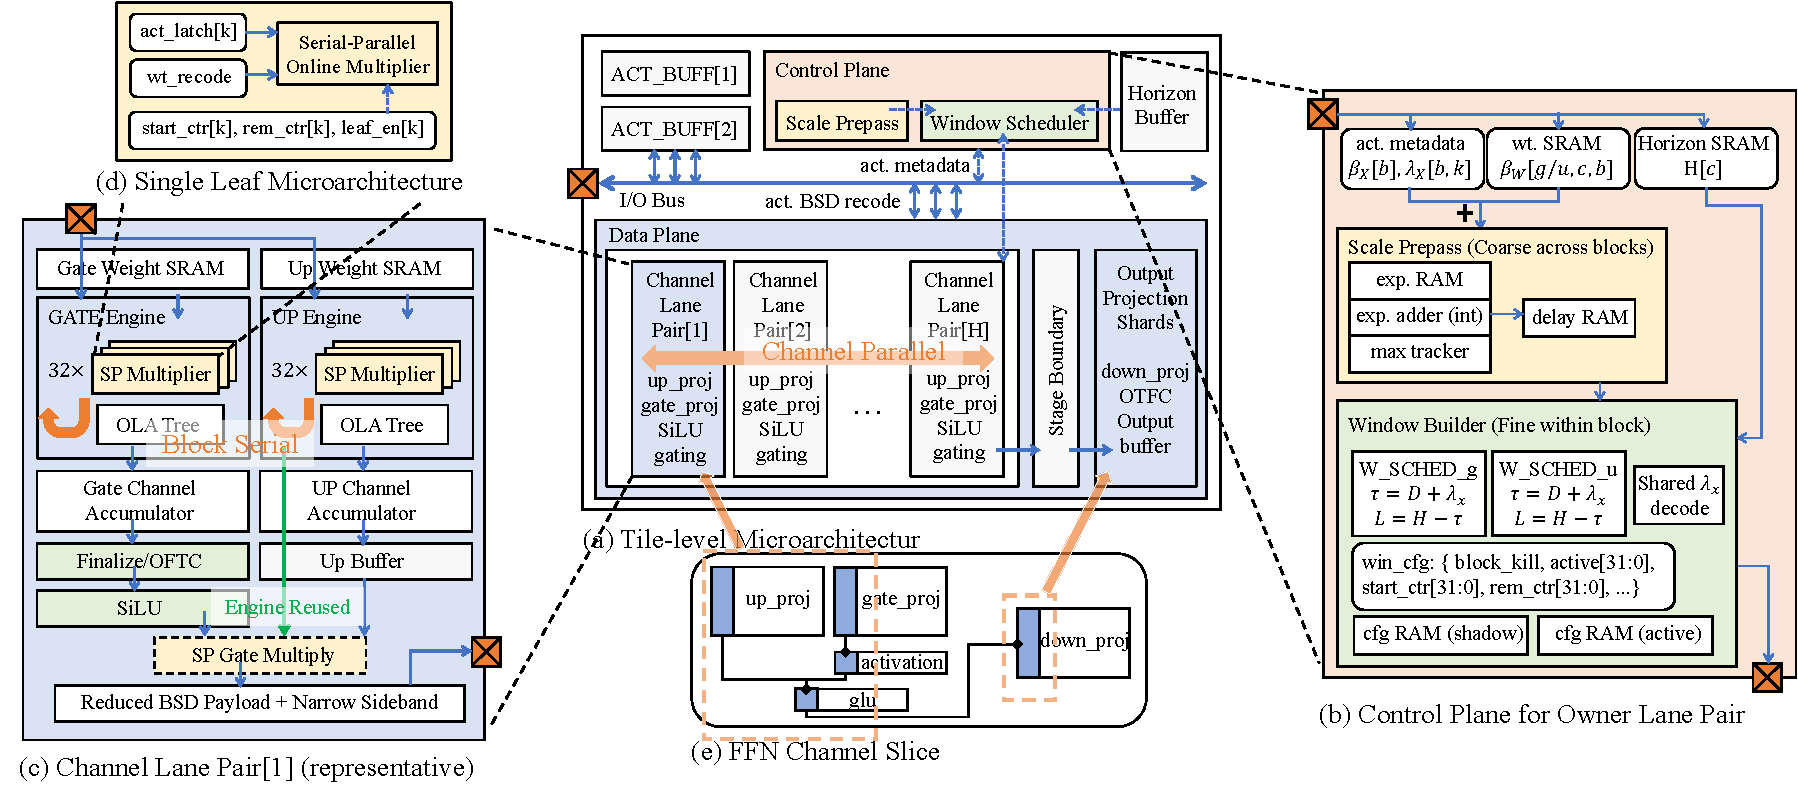
\includegraphics[width=\textwidth]{figures/figure3.pdf}
  \caption{%
    \textbf{Channel-parallel, block-serial two-plane FFN micro-tile.}}
  \label{fig:tile}
\end{figure*}

%% ======================================================================
%%  Section 4 — Hardware Realization
%% ======================================================================
\section{Hardware Realization}
\label{sec:hardware}
Figure~\ref{fig:tile} illustrates the proposed \textbf{metadata-first two-plane FFN micro-tile}, which realizes the scheduling strategy from Section~\ref{sec:method} with minimal hardware overhead. The tile design employs a weight-stationary Digital Compute-In-Memory (CIM) architecture: weight SRAM is locally integrated within every projection lane, with only the activation contribution streams traveling through the compute array. 

%% --------------------------------------------------
\subsection{Tile-Level FFN Mapping}
\label{sec:tile}
The proposed micro-tile maps the GLU-FFN onto three execution stages guided by a \emph{channel-parallel, block-serial} execution strategy (Figure~\ref{fig:tile}a):
\begin{enumerate}[nosep,leftmargin=1.2em]
  \item \textbf{Front-end projections.} The $W_{\mathrm{gate}}$ and $W_{\mathrm{up}}$ computations execute concurrently within channel-parallel projection lanes, while the $B$ input blocks assigned to each channel are serialized in time.
  \item \textbf{Local gating.} The SiLU nonlinearity and element-wise product ($\phi(\mathrm{gate}) \odot \mathrm{up}$) are evaluated directly on the intermediate results using a reused serial--parallel multiplier.
  \item \textbf{Output projection.} The gated output is forwarded to $S$ local $W_{\mathrm{down}}$ shards to compute the final projection.
\end{enumerate}

%% --------------------------------------------------
\subsection{Metadata-First Control Plane}
\label{sec:control}
By operating predominantly on metadata, the control plane enforces TSS with a minimal area footprint.

\textbf{Scale prepass.}
A metadata-only scan computes the cross-block maximum exponent $E_{\max}$ and resolves coarse block delays. This prepass strictly accesses narrow metadata arrays ($\beta_x$ and $\beta_w$) and low-bitwidth adders to update local registers, entirely bypassing the activation streams and Digital-CIM weight arrays.

\textbf{Shared $\lambda_x$ decode.}
The activation fine-delay vector $\lambda_x[n,b,0\!:\!31]$ is decoded once in a shared central cluster and broadcast to the relevant projection lanes.

\textbf{Per-lane window builders.}
Each lane combines the shared fine-delay vector with its local coarse delay and channel horizon to parameterize the per-element window configurations ($\tau$ and $L$, as defined in Section~\ref{sec:method}). These window limits are double-buffered locally, allowing the control logic to continuously prepare block $b\!+\!1$ while block $b$ executes.

%% --------------------------------------------------
\subsection{Online-Arithmetic Data Plane}
\label{sec:dataplane}
Exploiting the weight-stationary CIM substrate, each projection lane houses two block-processing engines corresponding to the front-end \texttt{gate\_proj} and \texttt{up\_proj}. Each engine comprises $K\!=\!32$ serial--parallel (SP) multiplier leaves, a five-level block-local overlap-add (OLA) reduction tree, and a channel accumulator that merges successive serialized blocks:
\begin{equation*}
  \mathrm{acc}[p,b\!+\!1,c]
    = \mathrm{OLA}\!\bigl(\mathrm{acc}[p,b,c],\;
                          s_{\mathrm{blk}}[p,b,c]\bigr).
\end{equation*}

After both accumulators finish, standard fixed-point logic applies the $\operatorname{SiLU}$ activation and evaluates $\text{gated}_c = \operatorname{SiLU}(\text{gate}_c)\odot\text{up}_c$. This intermediate result is passed to the local \texttt{down\_proj} shards, which contain dedicated SP multiplier banks and row accumulators. By passing windowed data streams directly alongside sideband metadata, this interface seamlessly connects the stages without requiring wide, full-precision buses.

%% --------------------------------------------------
\subsection{Hardware Savings via Operation Gating}
\label{sec:turnoff}
The three scheduling outcomes derived in Section~\ref{sec:method} directly translate into dynamic hardware savings:
\begin{itemize*}[nosep,leftmargin=1.2em]
    \item \textbf{Whole-block skips} entirely bypass the local arithmetic trees and corresponding memory reads, proportionally contracting the elapsed block execution span. 
    \item For \textbf{element skips} and \textbf{partial-window execution}, idle SP multiplier leaves and their local memory interfaces are clock-gated. Furthermore, inactive OLA-tree ancestors are dynamically gated once their residual states drain, consistently reducing switching activity even if the maximal block baseline interval remains unchanged.
\end{itemize*}
%% ======================================================================
%%  Section 5 — Experimental Methodology
%% ======================================================================

\section{Experimental Methodology}
\label{sec:setup}

This section details the simulation infrastructure, target models, hardware 
measurement methodology, and evaluation protocols that underpin the empirical 
results presented in Section~\ref{sec:results}.

%% --------------------------------------------------
\textbf{Transaction-Level Simulation.} We developed a custom open-source Python-based transaction-level model (TLM)~\cite{cai2003transaction,aguirre2024hardware} to simulate the 
precise MSD-first data flow of the proposed micro-tile 
(Section~\ref{sec:hardware}). The TLM tracks all serial-parallel 
multiplications, block-local overlap-add reductions, and channel accumulations 
at digit-level granularity. It reproduces the aligned contribution streams 
(Eq.~\ref{eq:sexec}) and windowed execution on a cycle-by-cycle basis. To 
ensure bit-exact numerical outputs with respect to the hardware scheduling 
abstraction, the TLM strictly avoids the use of floating-point surrogates 
within the inner loop.

%% --------------------------------------------------
\textbf{Model Setup and Calibration.} We evaluate our architecture using the Qwen3-0.6B model~\cite{yang2025qwen3} from the HuggingFace 
Transformers library~\cite{wolf2020huggingface}. To isolate the architectural effects of the feed-forward 
network (FFN), all experiments target the GLU-style FFN sublayers while 
keeping the attention sublayers at the dense baseline. 

Both weights and activations are quantized to the MXFP8 format (8-bit MX 
microscaling with E8M0 block-scale exponents and a block size of $K\!=\!32$). 
Block-scale exponents, activation fine-delay codes, and weight element 
exponents are extracted directly from this MX representation. An offline 
recoding process stores the aligned weight mantissa in a fixed-point format. Horizon calibration leverages a held-out set of 1024 tokens 
randomly sampled from the WikiText-2 training split, whereas all model 
quality metrics are evaluated on the disjoint WikiText-2 test split.


\begin{figure*}[htbp]
  \centering
  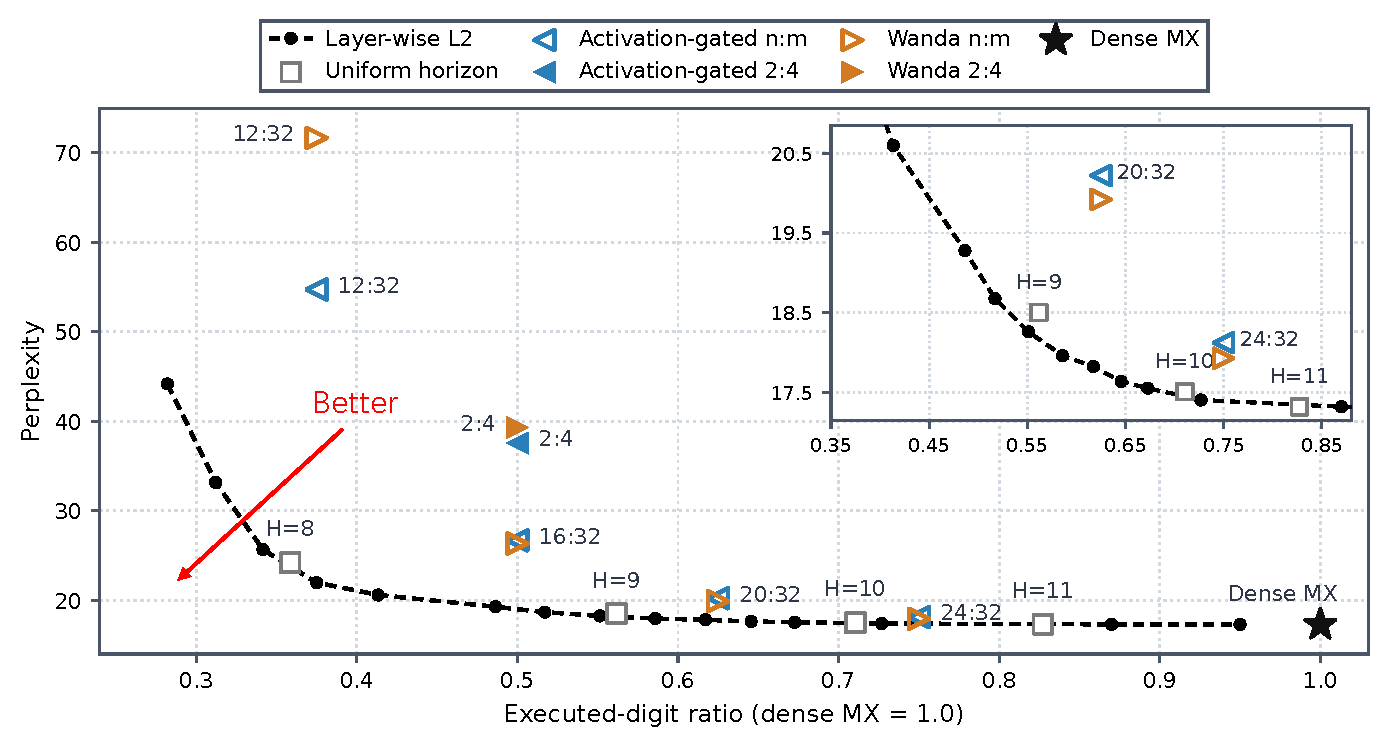
\includegraphics[width=0.8\textwidth]{figures/figure4.pdf}
  \caption{Quality-compute Pareto frontier for MX-quantized Qwen3-0.6B FFN inference.}
  \label{fig:pareto}
\end{figure*}

%% --------------------------------------------------
\textbf{Hardware Measurement Flow.} Our hardware measurement flow combines direct circuit implementation with 
macro-level modeling at the 28\si{nm} technology node. To evaluate area and 
power accurately, we partition the hardware into three distinct components: 
the control plane, the compute-in-memory (CIM) data plane, and SRAM storage.

The \emph{control plane} 
encompasses the complete TSS runtime scheduling logic and Horizon SRAM. We implement the control plane in Cadence Virtuoso and validate each component with transistor-level simulation in a commercial 28 \si{nm} process. This includes the 
metadata scale prepass (computing $E[b]$ and $E_{\max}$ from $\beta_x$ and 
$\beta_w$), the shared $\lambda_x$ decode/broadcast logic, per-lane window 
builders (forming $\tau$ and $L$ for horizon comparison), and all associated 
local registers and control logic. 

The CIM data plane—comprising the serial-parallel multipliers ~\cite{usman2023low}, overlap-add 
reduction trees, and channel accumulators—is synthesized using the Synopsys Design Compiler at a 28~\si{nm} technology node. Finally, weight 
storage is synthesized as SRAM macros using an ARM memory compiler for the 
same 28 \si{nm} node. The total reported per-channel area and power represent the 
direct sum of these three partitions.

%% --------------------------------------------------
\textbf{Baselines and Comparison Protocol.} All evaluated methods, including baselines, are normalized to a matched 
executed-digit ratio, defined as $\rho_{\mathrm{exec}} = N_{\mathrm{exec}} / N_{\mathrm{exec,dense}}$. We compare our proposed architecture against three baseline methodologies:
\begin{enumerate*}[nosep,leftmargin=1.2em]
  \item \textbf{Dense MXFP8 Baseline}: Full MXFP8 execution with no compute 
        suppression, serving as the primary dense anchor.
        
  \item \textbf{Dynamic Activation-Gated CIM}: Methods that apply fixed, 
        local masks derived dynamically from runtime activation statistics. 
        (~\cite{jeong2023vegeta,mishra2021accelerating}).
        
  \item \textbf{Static Calibrated Pruning}: A calibration-based static pruning baseline (Wanda~\cite{sun2023simple}) without retraining. This serves as the primary comparative baseline for our 
        calibrated layer-wise $L_2$ redistribution variant.
\end{enumerate*}

We map the resulting 
$n\!:\!m$ sparsity structure directly to the equivalent executed-digit ratio by $\rho_{\mathrm{exec}}=n/m$. 
For the proposed architecture, we evaluate three operating configurations: 
\emph{uniform horizon} (a baseline staircase anchor), \emph{channel-wise 
SNR-based redistribution} (an ablation variant), and \emph{layer-wise $L_2$ 
redistribution} (which establishes our main Pareto frontier).

%==================================================
\section{Evaluation Results}
\label{sec:results}
%==================================================

Our evaluation isolates the numerical fidelity of temporal significance scheduling before demonstrating its system-level benefits. We establish the quality-compute Pareto frontier, quantify the architectural benefits of reducing executed digits, validate the offline-online partitioning, and report the hardware efficiency.


\begin{figure}[htbp]
  \centering
  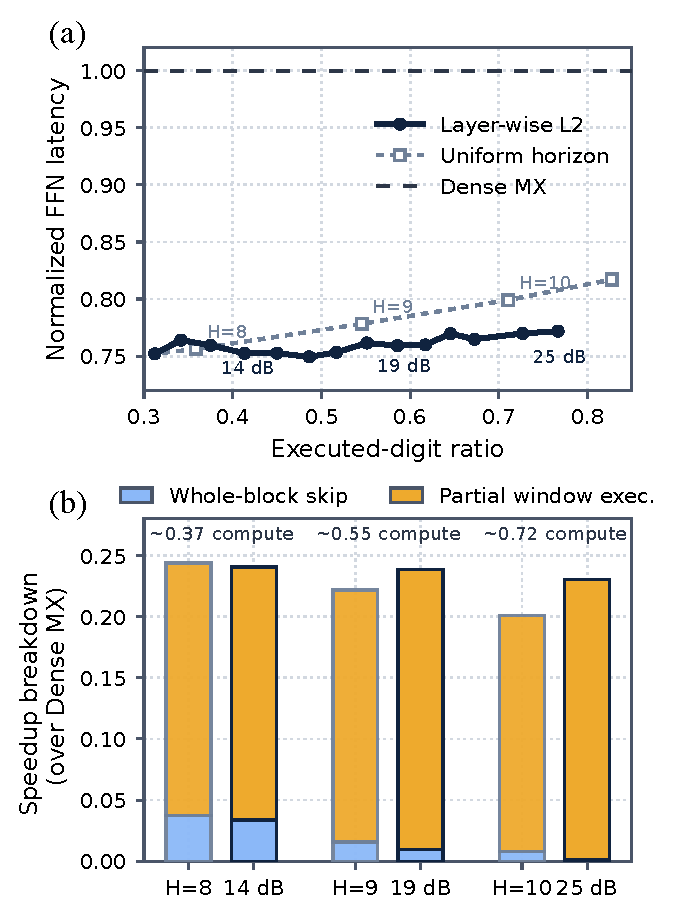
\includegraphics[width=0.9\linewidth]{figures/figure5.pdf}
  \caption{%
    (a)~Normalized FFN latency versus executed-digit ratio.
    (b)~Acceleration contribution breakdown.}
  \label{fig:layer_latency}
\end{figure}

\subsection{Core Quality-compute Pareto Frontier}
\label{sec:pareto}

Figure~\ref{fig:pareto} presents the quality-compute trade-off across all baseline configurations.

\textbf{Pareto efficiency of TSS.}
Across all executed-digit ratios, layer-wise $L_2$ redistribution consistently achieves the lowest perplexity, converging to the dense MX baseline as the ratio approaches 1.0. The discrete operating points of the uniform horizon policy fall along this same curve, indicating that quality improvements stem primarily from the TSS abstraction itself---specifically, executing local windows on aligned contribution streams. The redistribution mechanism interpolates between integer-horizon steps to provide fine-grained budget control, rather than fundamentally shifting the Pareto frontier.

\textbf{Comparison with structured sparsity.}
The widely adopted $2{:}4$ structured sparsity pattern yields substantially higher perplexity for both the online activation-gated mask and the Wanda, reflecting the limitations of coarse, fixed local patterns at this quantization level. Relaxing the constraint to an $n{:}32$ pattern improves quality by expanding the selection scope, but layer-wise $L_2$ redistribution consistently outperforms it at equivalent compute budgets. This performance gap widens at low executed-digit ratios, where preserving the most significant contributions under a tight budget is especially important.


\subsection{Layer-Wise Latency under Block-Serial Execution}
\label{sec:layer_latency}

Figure~\ref{fig:layer_latency} translates the projected compute reduction into realized FFN latency under a channel-parallel, block-serial execution model.



\textbf{Stable layer-level acceleration.}
As shown in Figure~\ref{fig:layer_latency}(a), layer-wise $L_2$ redistribution reduces normalized FFN latency by 22--25\% across the practical operating range. At higher executed-digit ratios, where the uniform horizon approach yields diminishing returns, layer-wise redistribution maintains a distinct advantage via fine-grained reallocation: channels contributing heavily to output quality retain higher precision, while less significant channels receive shorter service windows.

\textbf{Acceleration breakdown.}
Figure~\ref{fig:layer_latency}(b) breaks down this latency reduction. Whole-block skipping unconditionally eliminates block slots, providing a bounded acceleration that peaks at approximately 20\% of the total gain. The majority of savings stem from partial-window execution contracting the maximal live interval within partially executed blocks; this effect dominates at higher executed-digit ratios. As average horizons widen, fewer blocks qualify for full skips, yet partial-window contraction remains highly effective because individual contribution streams often initiate late relative to the channel horizon.

These results validate the architectural claims from Section~\ref{sec:method}: while whole-block skipping reduces block slots, partial-window execution reduces overall executed digits. In practice, these dual mechanisms yield substantial layer-level latency reductions as live intervals contract concurrently across multiple channels.

\subsection{Validation of the Offline-Online Partitioning}
\label{sec:offline_online}

Our design statically stores calibrated horizons and dynamically synthesizes local execution windows at runtime. Figure~\ref{fig:offline_online} validates three key properties of this offline-online split. First, regarding \textbf{budget controllability} (Figure~\ref{fig:offline_online}a), layer-wise $L_2$ redistribution provides near-linear, fine-grained tuning of the executed-digit ratio across the practical 0.3--0.7 regime, unlike the coarse step-function of a uniform horizon. Second, \textbf{calibration} is highly robust (Figure~\ref{fig:offline_online}b); model quality stabilizes with only ${\sim}1\text{k}$ calibration tokens---fewer than Wanda's requirement of 256 sequence samples, each containing $2\text{k}$ tokens~~\cite{sun2023simple}---because the lightweight procedure merely redistributes pre-existing budgets based on layer-level statistics. Finally, the \textbf{metadata-source ablation} (Figure~\ref{fig:offline_online}c) confirms that dynamic activation statistics are critical. Weight-only redistribution severely degrades perplexity ($>10^3$), whereas combining global activation and weight metadata (\emph{layer-wise} redistribution) achieves the lowest perplexity, outperforming independent \emph{channel-wise} optimization by ${\sim}1.6$ points.

\begin{figure}[htbp]
  \centering
  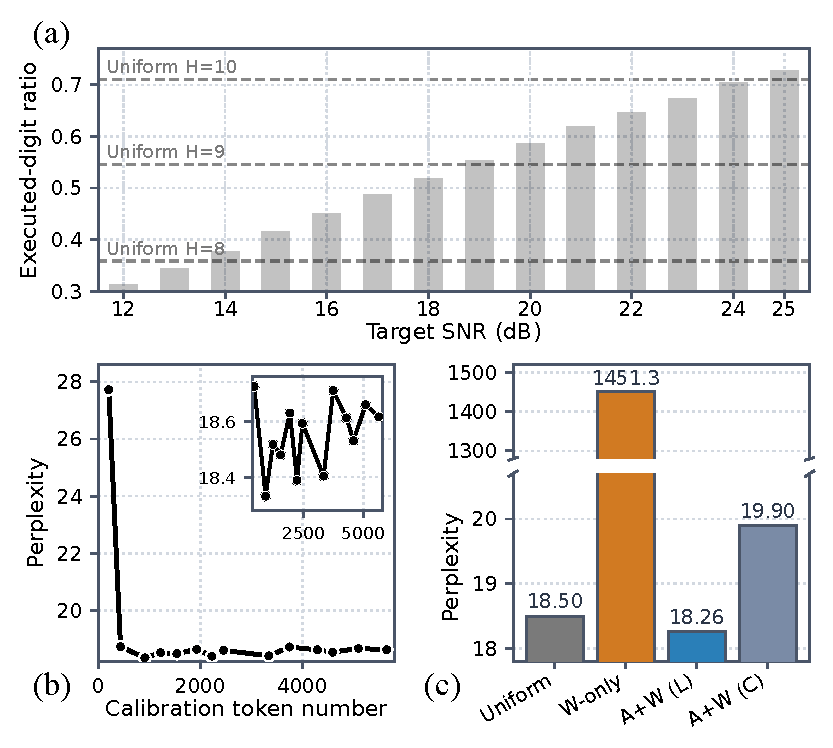
\includegraphics[width=\linewidth]{figures/figure6.pdf}
  \caption{%
    Validation of the offline-online split.
    (a)~Executed-digit ratio versus initialization target SNR for layer-wise $L_2$ redistribution and uniform horizon.
    (b)~Perplexity versus calibration sample size.
    (c)~Metadata-source ablation.}
  \label{fig:offline_online}
\end{figure}

\subsection{Hardware Cost}
\label{sec:hardware_cost}

Figure~\ref{fig:hw_breakdown} details the per-channel area and power breakdown of the synthesized hardware design across four functional domains.

\begin{figure}[htbp]
  \centering
  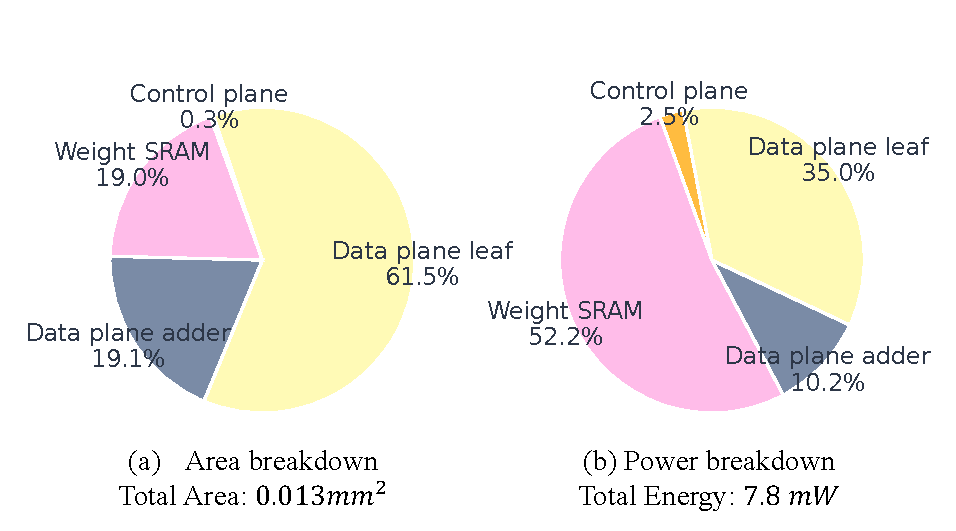
\includegraphics[width=\linewidth]{figures/figure7.pdf}
  \caption{%
    Per-channel area and power breakdown.}
  \label{fig:hw_breakdown}
\end{figure}

\textbf{Negligible Control-Plane Overhead.}
The control plane consumes just 45.1\,\si{\micro m^2} ($<$0.35\% of the 13\,008\,\si{\micro m^2} total per-channel area) and 0.198\,\si{mW} (${\approx}\,$2.5\% of the 7.81\,\si{mW} power budget). This validates our core architectural claim: replacing per-element spatial masks with per-channel horizons and block-level control reduces routing complexity from an $O(n)$ multiplexing network to lightweight scalar logic. Consequently, the control overhead is lower than that of representative spatial-sparsity accelerators.

\textbf{Data-Plane and SRAM Costs.}
The online arithmetic leaf dominates the area footprint (7\,996.6\,\si{\micro m^2}, 61.5\%) due to the digit-serial multiply--accumulate datapath required for MX-format computation. The adder tree accounts for 19.1\% of area and 10.3\% of power. The weight SRAM occupies 19.0\% of area and dictates overall power consumption (4.07\,\si{mW}, 52.2\%), reflecting the memory-intensive profile typical of compute-in-memory (CIM) macro designs. Crucially, the proposed scheduling policy strictly confines overhead to the control plane, leaving the adder tree and SRAM costs uninflated.

\begin{table}[htbp]
  \centering
  \caption{%
    \textbf{Comparison with relative hardware overheads of sparsity-aware accelerators.} 
    Control overhead denotes the area fraction attributed to sparsity and 
    scheduling logic. Prior values are quoted as reported in their respective 
    publications. For TSS, the value is calculated as the synthesized control-plane 
    area divided by the total per-channel tile area.}
  \label{tab:hw_comparison}
  \small
  \begin{tabular}{@{}lccc@{}}
    \toprule
    \textbf{Architecture} & \textbf{Policy} & \textbf{Precision} & \textbf{Control Overhead} \\
    \midrule
    Z.Yue~\cite{10904702}          & Activation 2:4   & FP16  & 26.0\% \\
    VEGETA~\cite{jeong2023vegeta}            & Flexible $n{:}m$ & BF16  & 15.4\% \\
    FlexCIM~\cite{mishra2021accelerating}           & Flexible $n{:}m$ & INT8  & 5.9\% \\
    SDP~\cite{tu2022sdp}               & Activation 1:2   & INT16 & 3.5\% \\
    \textbf{TSS (ours)} & \textbf{TSS}   & \textbf{MXFP8} & \textbf{0.35\%} \\
    \bottomrule
  \end{tabular}
\end{table}

\textbf{Comparison with Prior Accelerators.}
Table~\ref{tab:hw_comparison} contextualizes the TSS control overhead against recent sparsity-aware CIM and near-memory accelerators implemented in comparable (\SI{\le 28}{\nano\meter}) nodes. By dividing the synthesized control-plane area by the total per-channel tile area ($45.1\,\si{\micro\meter\squared} / 13{,}008\,\si{\micro\meter\squared}$), TSS demonstrates a control overhead of just 0.35\%. As shown, this result suggests materially lower control-area cost than spatial sparsity support logic.


%========================================================
\section{Conclusion}
\label{sec:conclusion}
%========================================================

Existing spatial sparsity methods inherently clash with the strict structural regularity demanded by compute-in-memory (CIM) architectures. To resolve this tension, we introduce \emph{Temporal Significance Scheduling (TSS)}, an execution paradigm that shifts significance-aware compute reduction from the spatial domain to the temporal domain. By repurposing native Microscaling (MX) block- and element-scale exponents as arrival-time signals within a most-significant-digit (MSD)-first arithmetic stream, our approach dynamically truncates low-significance operations without imposing divergent control flows on the underlying hardware array.

Empirical and physical synthesis results validate the architectural viability of this temporal abstraction. Implemented via a metadata-first, two-plane micro-tile, the required scheduling logic is entirely decoupled from the high-precision datapath, dictating a negligible overhead of 0.3\% in area and 2.5\% in power. When evaluated on the MXFP8-quantized Qwen3-0.6B model, our design achieves a 22--25\% FFN latency reduction. By establishing a superior quality-compute Pareto frontier compared to conventional activation-gated and static weight pruning baselines---all without requiring model retraining---this work demonstrates that the temporal dimension of digit-serial CIM execution provides a low-overhead, natively regular mechanism for dynamic compute suppression in modern LLM accelerators.


\bibliographystyle{ACM-Reference-Format}
\bibliography{reference}


\end{document}

